\documentclass[twocolumn]{article}

%% Language and font encodings
\usepackage[english]{babel}
\usepackage[utf8]{inputenc}
\usepackage{csquotes}
\bibliographystyle{unsrt}
\usepackage{booktabs}

\usepackage{tabu}
\usepackage[T1]{fontenc}

%% Sets page size and margins
\usepackage[a4paper,top=2cm,bottom=2cm,left=3cm,right=3cm,marginparwidth=1.75cm]{geometry}

%% Useful packages
\usepackage{amsmath}
\usepackage{graphicx}
%\usepackage{apacite}
\usepackage[colorinlistoftodos]{todonotes}
\usepackage[colorlinks=true, allcolors=blue]{hyperref}

\title {Project: Detecting failing computer servers on a network}
\author{B. Shadrack Jabes}
\date{\it{\today}}

\begin{document}
\maketitle

\section{Introduction}
The aim of this project is to write an algorithm to detect the anomalous behavior in computer servers. There are about 307 servers and as the computer servers are functioning two features of the server's are observed: 1. latency which determines transfer speed (ms) of contents within a pipe from the client to the server and back, 2. Throughput of the server (mb/s) which determines the amount of data transferred within a period of time. I build a gaussian model as a function of these two features of the server. I then visualize the density estimation from this gaussian model using an evaluation metric $\epsilon$ and identify the anomalous server. Thus using this anomaly detection algorithm one can identify the anomalous server within the dataset.

\section{Identifying features}
The dataset consists of two features of the server they are throughput (mb/s) and latency (ms). There are a total of 307 servers from which this data is collected. Majority of the servers operate normaly and only few exceptional servers may require the attention of the system administrator (see figure \ref{fig:dataset}).
                \begin{figure}
                \centering
                \includegraphics[clip=true,trim=0cm 0cm 0cm 0cm,width=8cm]{dataset.ps}\\
			\caption{Latency and throughput are the features of the computer server collected over 307 servers.}
                \label{fig:dataset}
                \end{figure}
		\section{Density estimation: Gaussian model}
		Firstly I compute the total probability density, $p(X)$, where $X$ are the features of the computer server. The total probability density, $p(X)$ can be written as the product of probability densities of individual features. To obtain the probability densities of individual features we fit each feature $X$ to a gaussian model and estimate the gaussian parameters correspoinding to each feature. Here we assume that each feature is independent therefore can be fitted with a gaussian model. Once we obtain the probability densities of individual features we take the product of each probability densities and compute the total probability density $p(x)$ as follows:
		\begin{equation}
			p(X) = \prod_{j=1}^{n}P(X_j;\mu_j,\sigma^2_j)
		\end{equation}
		where $n$ is the number of features, $\mu$ and $\sigma^2$ are the mean and the corresponding variance of the features. The mean and variance of each feature $i$ over the total number of servers $j$ are computed as follows:
		\begin{align}
			\mu = \frac{1}{m}\sum_{j=1}^{m}X^{(j)} \\
			\sigma^2_i = \frac{1}{m}\sum_{j=1}^m (X^{(j)} - \mu_j)^2
		\end{align}
			Where $m$ are the total number of servers.  
                \begin{figure}
                \centering
                \includegraphics[clip=true,trim=0cm 0cm 0cm 0cm,width=8cm]{contour.ps}\\
			\caption{Contour plot showning the probability density and the features.}
                \label{fig:dataset}
                \end{figure}
\section{Evaluation metric: $\epsilon$}
We now select the evaluation metric for the probability density and predict the anomaly such that if the probability density is below $\epsilon$ then the chances that the server is anomalous (flaged as $y=1$), else categorize the servers to be normal (flagged as $y=0$). To do that one needs to estimate the threshold $\epsilon$. The problem here is that the data set is skeweed, that is we have more examples with features that are normal and only fewer examples that are anomalous. Therefore from the dataset I evaluate F1-score for various choice of threshold $\epsilon$. I choose the $\epsilon$ valuse that corresponds to a high F1-score. The F1-score can be estimated as follow:
\begin{equation}
	F1 = \frac{2*P*R}{P+R}
\end{equation}
Here, precision, $P=\frac{tp}{tp+fp}$ and recall, $R = \frac{tp}{tp+fn}$. The $tp$,$fp$ and $fn$ are true positive, false positve and false negative respectively. True positive (tp): (i.e.,) when the actual label is anomalous but our gaussian model $p(X) < \epsilon$ predicts it correctly to be anomaly. False positve (fp): (i.e.,) when the actual label is anomalous but our gaussian model $p(X) < \epsilon$ predicts it falsely to be an anomaly. False negative (fn): (i.e.) when the actual label is anomalous but our gaussian model $p(X) < \epsilon$ predicts it falsely to be normal.
                \begin{figure}
                \centering
                \includegraphics[clip=true,trim=0cm 0cm 0cm 0cm,width=8cm]{model.ps}\\
			\caption{Detecting failing computer servers on a network}
                \label{fig:main}
                \end{figure}
\section{Contribution}
My contribution to this project is writting a high level vectorized programming code in {\it Octave} to estimate the parameters for the gaussian model and to find the best evaluation metric.
\end{document}
